\documentclass[12pt,a4paper]{article}

\usepackage[a4paper,text={16.5cm,25.2cm},centering, margin=1in]{geometry}

\usepackage[scale=0.95]{FiraMono}
\usepackage[utf8]{inputenc}
\usepackage[T1]{fontenc}
\usepackage{mathpazo}

\usepackage{amssymb,amsmath}
\usepackage{bm}
\usepackage{graphicx}
\usepackage{microtype}
\usepackage{hyperref}
\setlength{\parindent}{0pt}
\setlength{\parskip}{1.2ex}

\usepackage{fvextra}
\DefineVerbatimEnvironment{Highlighting}{Verbatim}{breaklines,commandchars=\\\{\}}

\setcounter{secnumdepth}{0}

\hypersetup
       {   pdfauthor = { Andrew Scacchi (ADS339) },
           pdftitle={ BEE 4750/5750 Homework 4 },
           colorlinks=TRUE,
           linkcolor=black,
           citecolor=blue,
           urlcolor=blue
       }

\title{ BEE 4750/5750 Homework 4 }

\author{ Andrew Scacchi (ADS339) }

\date{ 2022-11-04 }

\usepackage{upquote}
\usepackage{listings}
\usepackage{xcolor}
\lstset{
    basicstyle=\ttfamily\footnotesize,
    upquote=true,
    breaklines=true,
    breakindent=0pt,
    keepspaces=true,
    showspaces=false,
    columns=fullflexible,
    showtabs=false,
    showstringspaces=false,
    escapeinside={(*@}{@*)},
    extendedchars=true,
}
\newcommand{\HLJLt}[1]{#1}
\newcommand{\HLJLw}[1]{#1}
\newcommand{\HLJLe}[1]{#1}
\newcommand{\HLJLeB}[1]{#1}
\newcommand{\HLJLo}[1]{#1}
\newcommand{\HLJLk}[1]{\textcolor[RGB]{148,91,176}{\textbf{#1}}}
\newcommand{\HLJLkc}[1]{\textcolor[RGB]{59,151,46}{\textit{#1}}}
\newcommand{\HLJLkd}[1]{\textcolor[RGB]{214,102,97}{\textit{#1}}}
\newcommand{\HLJLkn}[1]{\textcolor[RGB]{148,91,176}{\textbf{#1}}}
\newcommand{\HLJLkp}[1]{\textcolor[RGB]{148,91,176}{\textbf{#1}}}
\newcommand{\HLJLkr}[1]{\textcolor[RGB]{148,91,176}{\textbf{#1}}}
\newcommand{\HLJLkt}[1]{\textcolor[RGB]{148,91,176}{\textbf{#1}}}
\newcommand{\HLJLn}[1]{#1}
\newcommand{\HLJLna}[1]{#1}
\newcommand{\HLJLnb}[1]{#1}
\newcommand{\HLJLnbp}[1]{#1}
\newcommand{\HLJLnc}[1]{#1}
\newcommand{\HLJLncB}[1]{#1}
\newcommand{\HLJLnd}[1]{\textcolor[RGB]{214,102,97}{#1}}
\newcommand{\HLJLne}[1]{#1}
\newcommand{\HLJLneB}[1]{#1}
\newcommand{\HLJLnf}[1]{\textcolor[RGB]{66,102,213}{#1}}
\newcommand{\HLJLnfm}[1]{\textcolor[RGB]{66,102,213}{#1}}
\newcommand{\HLJLnp}[1]{#1}
\newcommand{\HLJLnl}[1]{#1}
\newcommand{\HLJLnn}[1]{#1}
\newcommand{\HLJLno}[1]{#1}
\newcommand{\HLJLnt}[1]{#1}
\newcommand{\HLJLnv}[1]{#1}
\newcommand{\HLJLnvc}[1]{#1}
\newcommand{\HLJLnvg}[1]{#1}
\newcommand{\HLJLnvi}[1]{#1}
\newcommand{\HLJLnvm}[1]{#1}
\newcommand{\HLJLl}[1]{#1}
\newcommand{\HLJLld}[1]{\textcolor[RGB]{148,91,176}{\textit{#1}}}
\newcommand{\HLJLs}[1]{\textcolor[RGB]{201,61,57}{#1}}
\newcommand{\HLJLsa}[1]{\textcolor[RGB]{201,61,57}{#1}}
\newcommand{\HLJLsb}[1]{\textcolor[RGB]{201,61,57}{#1}}
\newcommand{\HLJLsc}[1]{\textcolor[RGB]{201,61,57}{#1}}
\newcommand{\HLJLsd}[1]{\textcolor[RGB]{201,61,57}{#1}}
\newcommand{\HLJLsdB}[1]{\textcolor[RGB]{201,61,57}{#1}}
\newcommand{\HLJLsdC}[1]{\textcolor[RGB]{201,61,57}{#1}}
\newcommand{\HLJLse}[1]{\textcolor[RGB]{59,151,46}{#1}}
\newcommand{\HLJLsh}[1]{\textcolor[RGB]{201,61,57}{#1}}
\newcommand{\HLJLsi}[1]{#1}
\newcommand{\HLJLso}[1]{\textcolor[RGB]{201,61,57}{#1}}
\newcommand{\HLJLsr}[1]{\textcolor[RGB]{201,61,57}{#1}}
\newcommand{\HLJLss}[1]{\textcolor[RGB]{201,61,57}{#1}}
\newcommand{\HLJLssB}[1]{\textcolor[RGB]{201,61,57}{#1}}
\newcommand{\HLJLnB}[1]{\textcolor[RGB]{59,151,46}{#1}}
\newcommand{\HLJLnbB}[1]{\textcolor[RGB]{59,151,46}{#1}}
\newcommand{\HLJLnfB}[1]{\textcolor[RGB]{59,151,46}{#1}}
\newcommand{\HLJLnh}[1]{\textcolor[RGB]{59,151,46}{#1}}
\newcommand{\HLJLni}[1]{\textcolor[RGB]{59,151,46}{#1}}
\newcommand{\HLJLnil}[1]{\textcolor[RGB]{59,151,46}{#1}}
\newcommand{\HLJLnoB}[1]{\textcolor[RGB]{59,151,46}{#1}}
\newcommand{\HLJLoB}[1]{\textcolor[RGB]{102,102,102}{\textbf{#1}}}
\newcommand{\HLJLow}[1]{\textcolor[RGB]{102,102,102}{\textbf{#1}}}
\newcommand{\HLJLp}[1]{#1}
\newcommand{\HLJLc}[1]{\textcolor[RGB]{153,153,119}{\textit{#1}}}
\newcommand{\HLJLch}[1]{\textcolor[RGB]{153,153,119}{\textit{#1}}}
\newcommand{\HLJLcm}[1]{\textcolor[RGB]{153,153,119}{\textit{#1}}}
\newcommand{\HLJLcp}[1]{\textcolor[RGB]{153,153,119}{\textit{#1}}}
\newcommand{\HLJLcpB}[1]{\textcolor[RGB]{153,153,119}{\textit{#1}}}
\newcommand{\HLJLcs}[1]{\textcolor[RGB]{153,153,119}{\textit{#1}}}
\newcommand{\HLJLcsB}[1]{\textcolor[RGB]{153,153,119}{\textit{#1}}}
\newcommand{\HLJLg}[1]{#1}
\newcommand{\HLJLgd}[1]{#1}
\newcommand{\HLJLge}[1]{#1}
\newcommand{\HLJLgeB}[1]{#1}
\newcommand{\HLJLgh}[1]{#1}
\newcommand{\HLJLgi}[1]{#1}
\newcommand{\HLJLgo}[1]{#1}
\newcommand{\HLJLgp}[1]{#1}
\newcommand{\HLJLgs}[1]{#1}
\newcommand{\HLJLgsB}[1]{#1}
\newcommand{\HLJLgt}[1]{#1}


\begin{document}

\maketitle

%  This setups the environment and installs packages, but doesn't appear in the generated document 
%  You shouldn't need to modify this 


\section{Problem 1}
\subsection{Problem 1.1}

\begin{lstlisting}
(*@\HLJLcs{{\#}Processing}@*) (*@\HLJLcs{Costs}@*) (*@\HLJLcs{Given}@*)
(*@\HLJLn{DispoFacility}@*) (*@\HLJLoB{=}@*) (*@\HLJLp{[}@*)(*@\HLJLs{"{}Landfill"{}}@*)(*@\HLJLp{,}@*) (*@\HLJLs{"{}Recycling"{}}@*)(*@\HLJLp{,}@*) (*@\HLJLs{"{}Waste2Energy"{}}@*)(*@\HLJLp{]}@*)
(*@\HLJLn{FacilityCapacity}@*) (*@\HLJLoB{=}@*) (*@\HLJLp{[}@*)(*@\HLJLni{200}@*)(*@\HLJLp{,}@*)(*@\HLJLni{350}@*)(*@\HLJLp{,}@*)(*@\HLJLni{150}@*)(*@\HLJLp{];}@*) (*@\HLJLcs{{\#}}@*) (*@\HLJLcs{Mg/day}@*)
(*@\HLJLn{FixedCost}@*) (*@\HLJLoB{=}@*) (*@\HLJLp{[}@*)(*@\HLJLni{2000}@*)(*@\HLJLp{,}@*) (*@\HLJLni{1500}@*)(*@\HLJLp{,}@*) (*@\HLJLni{2500}@*)(*@\HLJLp{];}@*) (*@\HLJLcs{{\#}}@*) (*@\HLJLcs{{\$}/day}@*)
(*@\HLJLn{TippingFee}@*) (*@\HLJLoB{=}@*) (*@\HLJLp{[}@*)(*@\HLJLni{50}@*)(*@\HLJLp{,}@*) (*@\HLJLni{7}@*)(*@\HLJLp{,}@*) (*@\HLJLni{60}@*)(*@\HLJLp{];}@*) (*@\HLJLcs{{\#}}@*) (*@\HLJLcs{{\$}/Mg}@*)
(*@\HLJLn{RecyclingCost}@*) (*@\HLJLoB{=}@*) (*@\HLJLp{[}@*)(*@\HLJLni{0}@*)(*@\HLJLp{,}@*) (*@\HLJLni{45}@*)(*@\HLJLp{,}@*) (*@\HLJLni{0}@*)(*@\HLJLp{];}@*) (*@\HLJLcs{{\#}}@*) (*@\HLJLcs{{\$}/Mg}@*)

(*@\HLJLcs{{\#}Transportation}@*) (*@\HLJLcs{Metrics}@*) (*@\HLJLcs{Given}@*)
(*@\HLJLn{Transport}@*)(*@\HLJLoB{=}@*) (*@\HLJLnfB{1.5}@*)(*@\HLJLp{;}@*) (*@\HLJLcs{{\#}}@*) (*@\HLJLcs{Per}@*) (*@\HLJLcs{Mg-Km}@*)
(*@\HLJLn{City1}@*) (*@\HLJLoB{=}@*) (*@\HLJLp{[}@*)(*@\HLJLni{30}@*)(*@\HLJLp{,}@*) (*@\HLJLni{5}@*)(*@\HLJLp{,}@*) (*@\HLJLni{15}@*)(*@\HLJLp{];}@*) (*@\HLJLcs{{\#}City}@*) (*@\HLJLcs{1}@*) (*@\HLJLcs{distances}@*) (*@\HLJLcs{to}@*) (*@\HLJLcs{treatment}@*) (*@\HLJLcs{facilities}@*) (*@\HLJLcs{(km)}@*)
(*@\HLJLn{City2}@*) (*@\HLJLoB{=}@*) (*@\HLJLp{[}@*)(*@\HLJLni{25}@*)(*@\HLJLp{,}@*) (*@\HLJLni{15}@*)(*@\HLJLp{,}@*) (*@\HLJLni{10}@*)(*@\HLJLp{];}@*) (*@\HLJLcs{{\#}City}@*) (*@\HLJLcs{2}@*) (*@\HLJLcs{distances}@*) (*@\HLJLcs{(km)}@*)
(*@\HLJLn{MRF}@*) (*@\HLJLoB{=}@*) (*@\HLJLp{[}@*)(*@\HLJLni{32}@*)(*@\HLJLp{,}@*) (*@\HLJLni{0}@*)(*@\HLJLp{,}@*) (*@\HLJLni{15}@*)(*@\HLJLp{];}@*) (*@\HLJLcs{{\#}Distances}@*) (*@\HLJLcs{between}@*) (*@\HLJLcs{facilities}@*) (*@\HLJLcs{(km)}@*)
(*@\HLJLn{LF}@*) (*@\HLJLoB{=}@*) (*@\HLJLp{[}@*)(*@\HLJLni{0}@*)(*@\HLJLp{,}@*) (*@\HLJLni{32}@*)(*@\HLJLp{,}@*) (*@\HLJLni{18}@*)(*@\HLJLp{];}@*) (*@\HLJLcs{{\#}Distance}@*) (*@\HLJLcs{from}@*) (*@\HLJLcs{landfill}@*) (*@\HLJLcs{(km)}@*)
(*@\HLJLn{WTE}@*) (*@\HLJLoB{=}@*) (*@\HLJLp{[}@*)(*@\HLJLni{18}@*)(*@\HLJLp{,}@*) (*@\HLJLni{15}@*)(*@\HLJLp{,}@*) (*@\HLJLni{0}@*)(*@\HLJLp{];}@*) (*@\HLJLcs{{\#}Distance}@*) (*@\HLJLcs{from}@*) (*@\HLJLcs{waste}@*) (*@\HLJLcs{2}@*) (*@\HLJLcs{energy}@*) (*@\HLJLcs{(km)}@*)

(*@\HLJLcs{{\#}Waste}@*) (*@\HLJLcs{Input}@*) (*@\HLJLcs{Metrics}@*) (*@\HLJLcs{Given}@*)
(*@\HLJLn{Cities}@*) (*@\HLJLoB{=}@*) (*@\HLJLp{[}@*)(*@\HLJLs{"{}City}@*) (*@\HLJLs{1"{}}@*)(*@\HLJLp{,}@*) (*@\HLJLs{"{}City}@*) (*@\HLJLs{2"{}}@*)(*@\HLJLp{];}@*)
(*@\HLJLn{DSW}@*) (*@\HLJLoB{=}@*) (*@\HLJLp{[}@*)(*@\HLJLni{100}@*)(*@\HLJLp{,}@*) (*@\HLJLni{170}@*)(*@\HLJLp{];}@*) (*@\HLJLcs{{\#}Daily}@*) (*@\HLJLcs{solid}@*) (*@\HLJLcs{waste}@*) (*@\HLJLcs{produced}@*) (*@\HLJLcs{by}@*) (*@\HLJLcs{cities}@*) (*@\HLJLcs{(Mg)}@*)
(*@\HLJLn{I}@*) (*@\HLJLoB{=}@*) (*@\HLJLni{1}@*)(*@\HLJLoB{:}@*)(*@\HLJLni{2}@*)(*@\HLJLp{;}@*) (*@\HLJLcs{{\#}set}@*) (*@\HLJLcs{values}@*) (*@\HLJLcs{of}@*) (*@\HLJLcs{I}@*) (*@\HLJLcs{for}@*) (*@\HLJLcs{later}@*)
(*@\HLJLn{J}@*) (*@\HLJLoB{=}@*) (*@\HLJLni{1}@*)(*@\HLJLoB{:}@*)(*@\HLJLni{3}@*)(*@\HLJLp{;}@*) (*@\HLJLcs{{\#}set}@*) (*@\HLJLcs{values}@*) (*@\HLJLcs{of}@*) (*@\HLJLcs{J}@*) (*@\HLJLcs{for}@*) (*@\HLJLcs{later}@*)

(*@\HLJLn{Component}@*) (*@\HLJLoB{=}@*) (*@\HLJLp{[}@*)(*@\HLJLs{"{}Food}@*) (*@\HLJLs{Wastes"{}}@*)(*@\HLJLp{,}@*) (*@\HLJLs{"{}Paper}@*) (*@\HLJLs{{\&}}@*) (*@\HLJLs{Cardboard"{}}@*)(*@\HLJLp{,}@*) (*@\HLJLs{"{}Plastics"{}}@*)(*@\HLJLp{,}@*) (*@\HLJLs{"{}Textiles"{}}@*)(*@\HLJLp{,}@*) (*@\HLJLs{"{}Rubber/}@*) (*@\HLJLs{Leather"{}}@*)(*@\HLJLp{,}@*) (*@\HLJLs{"{}Wood"{}}@*)(*@\HLJLp{,}@*) (*@\HLJLs{"{}Yard}@*) (*@\HLJLs{Wastes"{}}@*)(*@\HLJLp{,}@*) (*@\HLJLs{"{}Glass"{}}@*)(*@\HLJLp{,}@*) 
(*@\HLJLs{"{}Ferrous"{}}@*)(*@\HLJLp{,}@*) (*@\HLJLs{"{}Aluminum"{}}@*)(*@\HLJLp{,}@*) (*@\HLJLs{"{}Other}@*) (*@\HLJLs{Metal"{}}@*)(*@\HLJLp{,}@*) (*@\HLJLs{"{}Miscellaneous"{}}@*)(*@\HLJLp{];}@*) (*@\HLJLcs{{\#}Listed}@*) (*@\HLJLcs{Solid}@*) (*@\HLJLcs{Waste}@*) (*@\HLJLcs{Types}@*) (*@\HLJLcs{Processed}@*)
(*@\HLJLn{PctTM}@*) (*@\HLJLoB{=}@*) (*@\HLJLp{[}@*)(*@\HLJLnfB{.15}@*)(*@\HLJLp{,}@*) (*@\HLJLnfB{.40}@*)(*@\HLJLp{,}@*) (*@\HLJLnfB{.05}@*)(*@\HLJLp{,}@*) (*@\HLJLnfB{.03}@*)(*@\HLJLp{,}@*) (*@\HLJLnfB{.02}@*)(*@\HLJLp{,}@*) (*@\HLJLnfB{.05}@*)(*@\HLJLp{,}@*) (*@\HLJLnfB{.18}@*)(*@\HLJLp{,}@*) (*@\HLJLnfB{.04}@*)(*@\HLJLp{,}@*) (*@\HLJLnfB{.02}@*)(*@\HLJLp{,}@*) (*@\HLJLnfB{.02}@*)(*@\HLJLp{,}@*) (*@\HLJLnfB{.01}@*)(*@\HLJLp{,}@*) (*@\HLJLnfB{.03}@*)(*@\HLJLp{];}@*) (*@\HLJLcs{{\#}Percent}@*) (*@\HLJLcs{of}@*) (*@\HLJLcs{total}@*) (*@\HLJLcs{mass}@*) (*@\HLJLcs{processed}@*)
(*@\HLJLn{CombustionAshPct}@*) (*@\HLJLoB{=}@*) (*@\HLJLp{[}@*)(*@\HLJLnfB{0.08}@*)(*@\HLJLp{,}@*) (*@\HLJLnfB{0.07}@*)(*@\HLJLp{,}@*) (*@\HLJLnfB{0.05}@*)(*@\HLJLp{,}@*) (*@\HLJLnfB{0.10}@*)(*@\HLJLp{,}@*) (*@\HLJLnfB{0.15}@*)(*@\HLJLp{,}@*) (*@\HLJLnfB{0.02}@*)(*@\HLJLp{,}@*) (*@\HLJLnfB{0.02}@*)(*@\HLJLp{,}@*) (*@\HLJLni{1}@*)(*@\HLJLp{,}@*) (*@\HLJLni{1}@*)(*@\HLJLp{,}@*) (*@\HLJLni{1}@*)(*@\HLJLp{,}@*) (*@\HLJLni{1}@*)(*@\HLJLp{,}@*) (*@\HLJLnfB{0.70}@*)(*@\HLJLp{];}@*) (*@\HLJLcs{{\#}Percent}@*) (*@\HLJLcs{of}@*) (*@\HLJLcs{combustion}@*) (*@\HLJLcs{that}@*) (*@\HLJLcs{turns}@*) (*@\HLJLcs{to}@*) (*@\HLJLcs{ash}@*)
(*@\HLJLn{MRFRecycle}@*) (*@\HLJLoB{=}@*) (*@\HLJLp{[}@*)(*@\HLJLni{0}@*)(*@\HLJLp{,}@*) (*@\HLJLnfB{0.55}@*)(*@\HLJLp{,}@*) (*@\HLJLnfB{0.15}@*)(*@\HLJLp{,}@*) (*@\HLJLnfB{0.10}@*)(*@\HLJLp{,}@*) (*@\HLJLni{0}@*)(*@\HLJLp{,}@*) (*@\HLJLnfB{0.30}@*)(*@\HLJLp{,}@*) (*@\HLJLnfB{0.40}@*)(*@\HLJLp{,}@*) (*@\HLJLnfB{0.60}@*)(*@\HLJLp{,}@*) (*@\HLJLnfB{0.75}@*)(*@\HLJLp{,}@*) (*@\HLJLnfB{0.80}@*)(*@\HLJLp{,}@*) (*@\HLJLnfB{0.50}@*)(*@\HLJLp{,}@*) (*@\HLJLni{0}@*)(*@\HLJLp{];}@*) (*@\HLJLcs{{\#}Percent}@*) (*@\HLJLcs{able}@*) (*@\HLJLcs{to}@*) (*@\HLJLcs{be}@*) (*@\HLJLcs{recycled}@*) (*@\HLJLcs{in}@*) (*@\HLJLcs{a}@*) (*@\HLJLcs{MRF}@*)


(*@\HLJLcs{{\#}Compute}@*) (*@\HLJLcs{Fractions}@*) (*@\HLJLcs{of}@*) (*@\HLJLcs{waste}@*) (*@\HLJLcs{streams}@*)
(*@\HLJLn{RecycleCoeff}@*) (*@\HLJLoB{=}@*) (*@\HLJLnf{sum}@*)(*@\HLJLp{(}@*)(*@\HLJLn{PctTM}@*) (*@\HLJLoB{.*}@*) (*@\HLJLn{MRFRecycle}@*)(*@\HLJLp{)}@*)
(*@\HLJLn{AshCoeff}@*) (*@\HLJLoB{=}@*) (*@\HLJLnf{sum}@*)(*@\HLJLp{(}@*)(*@\HLJLn{PctTM}@*)(*@\HLJLoB{.*}@*) (*@\HLJLn{CombustionAshPct}@*)(*@\HLJLp{)}@*)
(*@\HLJLn{XX}@*) (*@\HLJLoB{=}@*) (*@\HLJLnf{round}@*)(*@\HLJLp{(}@*)(*@\HLJLn{RecycleCoeff}@*)(*@\HLJLp{,}@*) (*@\HLJLn{digits}@*) (*@\HLJLoB{=}@*) (*@\HLJLni{4}@*)(*@\HLJLp{);}@*) (*@\HLJLcs{{\#}round}@*) (*@\HLJLcs{computed}@*) (*@\HLJLcs{values}@*)
(*@\HLJLn{YY}@*) (*@\HLJLoB{=}@*) (*@\HLJLnf{round}@*)(*@\HLJLp{(}@*)(*@\HLJLn{AshCoeff}@*)(*@\HLJLp{,}@*) (*@\HLJLn{digits}@*) (*@\HLJLoB{=}@*) (*@\HLJLni{4}@*)(*@\HLJLp{);}@*) (*@\HLJLcs{{\#}Round}@*) (*@\HLJLcs{computed}@*) (*@\HLJLcs{values}@*)

(*@\HLJLcs{{\#}Print}@*) (*@\HLJLcs{result}@*)
(*@\HLJLnf{println}@*)(*@\HLJLp{(}@*)(*@\HLJLs{"{}The}@*) (*@\HLJLs{overall}@*) (*@\HLJLs{recycling}@*) (*@\HLJLs{fraction}@*) (*@\HLJLs{of}@*) (*@\HLJLs{solid}@*) (*@\HLJLs{waste}@*) (*@\HLJLs{produced}@*) (*@\HLJLs{is}@*) (*@\HLJLs{"{}}@*)(*@\HLJLp{,}@*) (*@\HLJLn{XX}@*)(*@\HLJLp{);}@*)
(*@\HLJLnf{println}@*)(*@\HLJLp{(}@*)(*@\HLJLs{"{}The}@*) (*@\HLJLs{overall}@*) (*@\HLJLs{ash}@*) (*@\HLJLs{fraction}@*) (*@\HLJLs{of}@*) (*@\HLJLs{solid}@*) (*@\HLJLs{waste}@*) (*@\HLJLs{produced}@*) (*@\HLJLs{is}@*) (*@\HLJLs{"{}}@*)(*@\HLJLp{,}@*) (*@\HLJLn{YY}@*)(*@\HLJLp{);}@*)
\end{lstlisting}

The overall recycling fraction of solid waste produced is 0.3775
The overall ash fraction of solid waste produced is 0.1641


\subsection{Problem 1.2}
This problem appears to have three decision variables: 

\begin{itemize}
\item[1. ] The amount of waste (in Mg/day) transported from $City_i$ to $Facility_j$, denoted as $W_{i,j}$.


\item[2. ] How much residual waste (in Mg/day) is transported from the the Recycling facility to each of the other two

\end{itemize}
facilities for final disposal. This is denoted as $R_{k,j}$.

\begin{itemize}
\item[3. ] Whether any of the facilities will be operational on any given day, denoted by $O_j$, with $O$ being a standard boolean.

\end{itemize}
\subsection{Problem 1.3}
The given objective of this model is to dtermine an optimal disposal plan for the two cities,  i.e. find the disposal allocation that minimizes costs for the cities. To do this, the objective function needs to derive  the functions that govern the total cost (fixed and variable) for each of the three facilities. Then these three functions will be  combined into one total cost function, which will serve as the objective function subjected to constraints.

First, $C_{LF}$ will represent the cost of landfill disposal:

\[
C_{LF} = O_1*2000 + 50*(W_{1,1}+ W_{2,1} + R_{2,1} + R_{3,1}) + 1.5*(City1[1]*W_{1,1} + City2[1]* W_{2,1} + LF[2]*R_{1,2} + LF[3]*R_{1,3});
\]
Next, $C_{MRF}$ will represent the cost of the MRF:

\[
C_{MRF} = O_2*1500 + 7*(W_{1,2} + W_{2,2} + R_{1,2} + R_{3,2}) + (0.3775*45)*(W_{1,2} + W_{2,2} + R_{1,2} + R_{3,2})+ 1.5*(City1[2]*W_{1,2} + City2[2]*W_{2,2} + MRF[1]*R_{2,1} + MRF[3]*R_{2,3});
\]
Lastly, $C_{W2E}$ is the cost of the waste to energy recovery plant:

\[
C_{W2E} = O_3*2500 + 60*(W_{1,3} + W_{2,3} + R_{1,3} + R_{2,3}) + 1.5*(City1[3]*W_{1,3} + City2[3]*W_{2,3} + WTE[1]*R_{3,1} + WTE[2]*R_{3,2});
\]
Eliminating unnessesary terms and aggregating leaves the cost objective function:

\[
TC = O_1 * 2000 + O_2*1500 + O_3*2500 + 50*(W_{1,1}+ W_{2,1} + R_{2,1} + R_{3,1}) + 1.5*(City1[1]*W_{1,1} + City2[2]*W_{2,1}) + 7*(W_{1,2} + W_{2,2})+ (0.3775*45)*(W_{1,2} + W_{2,2})+
1.5*(City1[2]*W_{1,2} + City2[2]*W_{2,2} + MRF[1]*R_{2,1} + MRF[3]*R_{2,3}) + 60*(W_{1,3} + W_{2,3} + R_{2,3}) + 1.5*(City1[3]*W_{1,3} + City2[3]*W_{2,3} + WTE[1]*R_{3,1})
\]
Or simply:

\[
TC = Min(C_{LF} + C_{MRF} + C_{W2E})
\]
\subsection{Problem 1.4}
There are several constraints to ghis problem. In no order they are:

\begin{itemize}
\item[1. ] The sum of waste transported from each city to a facility adds up to the amount produced:

\end{itemize}
\[
\sum W_{1,j} = 100 ;
\sum W_{2,j} = 170 ;
\]
This ensures that waste WILL be produced and need to be processed in some way every day.

\begin{itemize}
\item[2. ] Recycling residuals from the MRF can only go to either the landfill or W2E plant, and the residual ash of the W2E plant must go the landfill.

\end{itemize}
\[
R_{1,1}, R_{1,2}, R_{1,3}, R_{2,2}, R_{3,2}, R_{3,3} = 0;
R_{3,1} = CombustionAshPercent * (W_{1,3} + W_{2,3} + R_{2,3});
\]
This eliminates violating any physical constraints on the treatments, including a facility sending waste to itself.

\begin{itemize}
\item[3. ] If no waste is going to a facility, then $O_j$ = 0

\end{itemize}
\[
Iff W_{1,1} + W_{2,1} + R_{2,1} + R_{3,1} = 0, O_1 = 0;
Iff W_{1,2} + W_{2,2} = 0, O_2 = 0;
Iff W_{1,3} + W_{2,3} + R_{2,3} = 0, O_3 = 0;
\]
In affect, this turns off the boolean and removes fixed costs from the equation.

\begin{itemize}
\item[4. ] Waste cannot be transported in a negative amount.

\end{itemize}
\[
W_{i,j} \geq 0;
R_{k,j} \geq 0;
\]
This means that msw can only flow in one direction.

\begin{itemize}
\item[5. ] A facility cannot handle more than its capacity.

\end{itemize}
\[
W_{1,1} + W_{2,1} + R_{2,1} + R_{3,1}\leq 200;
W_{1,2} + W_{2,2} \leq 350;
W_{1,3} + W_{2,3} + R_{2,3} \leq 150;
\]
\begin{itemize}
\item[6. ] Only unrecyclable MSW leaves the MRF, supporting the conservation of mass.

\end{itemize}
\[
R_{2,1} + R_{2,3} = (1-XX) * (W_{1,2} + W_{2,2})
\]
\begin{itemize}
\item[7. ] Ash that comes from recycled materials has a different combustion yield than virgin materials.

\end{itemize}
While the component of ash from virgin marterial can be denoted by:

\[
R_{3,1}^virgin = (YY) * (W_{1,3} + W_{2,3}) 
\]
Residual recycling has a different composition and ash rate that needs to be derived. This is done by finding the  material breakdown of materials that were unable to be recycled, and recomputing using the same methodology for the original calculation, as follows:


\begin{lstlisting}
(*@\HLJLn{RecycleOnes}@*) (*@\HLJLoB{=}@*) (*@\HLJLnf{ones}@*)(*@\HLJLp{(}@*)(*@\HLJLnf{length}@*)(*@\HLJLp{(}@*)(*@\HLJLn{MRFRecycle}@*)(*@\HLJLp{));}@*)
(*@\HLJLn{ResidualMasses}@*) (*@\HLJLoB{=}@*) (*@\HLJLn{PctTM}@*)(*@\HLJLoB{.*}@*)(*@\HLJLp{(}@*)(*@\HLJLn{RecycleOnes}@*)(*@\HLJLoB{-}@*)(*@\HLJLn{MRFRecycle}@*)(*@\HLJLp{);}@*)
(*@\HLJLn{NewMasses}@*) (*@\HLJLoB{=}@*) (*@\HLJLn{ResidualMasses}@*)(*@\HLJLoB{/}@*)(*@\HLJLp{(}@*)(*@\HLJLnf{sum}@*)(*@\HLJLp{(}@*)(*@\HLJLn{ResidualMasses}@*)(*@\HLJLp{));}@*)
(*@\HLJLn{NewAshContent}@*) (*@\HLJLoB{=}@*) (*@\HLJLnf{sum}@*)(*@\HLJLp{(}@*)(*@\HLJLn{NewMasses}@*)(*@\HLJLoB{.*}@*)(*@\HLJLn{CombustionAshPct}@*)(*@\HLJLp{)}@*)
\end{lstlisting}

0.13861044176706827


Meaning that 

\[
R_{3,1}^recovered = NewAshContent*R_{2,3};
\]
For an aggregate of:

\[
R_{3,1} = R_{3,1}^recovered + R_{3,1}^virgin;
=NewAshContent*R_{2,3} + (YY) * (W_{1,3} + W_{2,3}) 
\]
These are a complete set of constraints as all outlined constraints and physical limitations of the inputs, transportation of waste, and outputs have been accounted for. These constraints incorporate the concept of conservation of mass, and ensure that waste is only transported to where it makes sense.

\subsection{Problem 1.5}

\begin{lstlisting}
(*@\HLJLk{using}@*) (*@\HLJLn{JuMP}@*)
(*@\HLJLk{using}@*) (*@\HLJLn{Cbc}@*)

(*@\HLJLn{waste}@*) (*@\HLJLoB{=}@*) (*@\HLJLnf{Model}@*)(*@\HLJLp{(}@*)(*@\HLJLn{Cbc}@*)(*@\HLJLoB{.}@*)(*@\HLJLn{Optimizer}@*)(*@\HLJLp{)}@*)

(*@\HLJLcs{{\#}decision}@*) (*@\HLJLcs{variables}@*)
(*@\HLJLnd{@variable}@*)(*@\HLJLp{(}@*)(*@\HLJLn{waste}@*)(*@\HLJLp{,}@*) (*@\HLJLn{W}@*)(*@\HLJLp{[}@*)(*@\HLJLn{i}@*) (*@\HLJLkp{in}@*) (*@\HLJLn{I}@*)(*@\HLJLp{,}@*) (*@\HLJLn{j}@*) (*@\HLJLkp{in}@*) (*@\HLJLn{J}@*)(*@\HLJLp{]}@*) (*@\HLJLoB{\ensuremath{\geq}}@*) (*@\HLJLni{0}@*)(*@\HLJLp{)}@*)
(*@\HLJLnd{@variable}@*)(*@\HLJLp{(}@*)(*@\HLJLn{waste}@*)(*@\HLJLp{,}@*) (*@\HLJLn{R}@*)(*@\HLJLp{[}@*)(*@\HLJLn{k}@*) (*@\HLJLkp{in}@*) (*@\HLJLn{J}@*)(*@\HLJLp{,}@*) (*@\HLJLn{j}@*) (*@\HLJLkp{in}@*) (*@\HLJLn{J}@*)(*@\HLJLp{]}@*) (*@\HLJLoB{\ensuremath{\geq}}@*) (*@\HLJLni{0}@*)(*@\HLJLp{)}@*)
(*@\HLJLnd{@variable}@*)(*@\HLJLp{(}@*)(*@\HLJLn{waste}@*)(*@\HLJLp{,}@*) (*@\HLJLn{O}@*)(*@\HLJLp{[}@*)(*@\HLJLn{j}@*) (*@\HLJLkp{in}@*) (*@\HLJLn{J}@*)(*@\HLJLp{],}@*) (*@\HLJLn{Bin}@*)(*@\HLJLp{)}@*)

(*@\HLJLcs{{\#}define}@*) (*@\HLJLcs{objective}@*)
(*@\HLJLnd{@objective}@*)(*@\HLJLp{(}@*)(*@\HLJLn{waste}@*)(*@\HLJLp{,}@*) (*@\HLJLn{Min}@*)(*@\HLJLp{,}@*) (*@\HLJLnf{sum}@*)(*@\HLJLp{([}@*)(*@\HLJLni{2000}@*)(*@\HLJLp{,}@*)(*@\HLJLni{1500}@*)(*@\HLJLp{,}@*)(*@\HLJLni{2500}@*)(*@\HLJLp{]}@*)(*@\HLJLoB{.*}@*)(*@\HLJLn{O}@*)(*@\HLJLp{)}@*) (*@\HLJLoB{+}@*) (*@\HLJLnf{sum}@*)(*@\HLJLp{([}@*)(*@\HLJLni{95}@*) (*@\HLJLnfB{31.5}@*) (*@\HLJLnfB{82.5}@*)(*@\HLJLp{;}@*) (*@\HLJLnfB{87.5}@*) (*@\HLJLnfB{46.49}@*) (*@\HLJLni{75}@*)(*@\HLJLp{]}@*)(*@\HLJLoB{.*}@*)(*@\HLJLn{W}@*)(*@\HLJLp{)}@*) (*@\HLJLoB{+}@*) (*@\HLJLnf{sum}@*)(*@\HLJLp{([}@*)(*@\HLJLni{0}@*) (*@\HLJLni{0}@*) (*@\HLJLni{0}@*)(*@\HLJLp{;}@*) (*@\HLJLni{98}@*) (*@\HLJLni{0}@*) (*@\HLJLnfB{82.5}@*)(*@\HLJLp{;}@*) (*@\HLJLni{77}@*) (*@\HLJLni{0}@*) (*@\HLJLni{0}@*)(*@\HLJLp{]}@*)(*@\HLJLoB{.*}@*)(*@\HLJLn{R}@*)(*@\HLJLp{));}@*)

(*@\HLJLcs{{\#}Constraints}@*)
(*@\HLJLcs{{\#}Capacity}@*) (*@\HLJLcs{and}@*) (*@\HLJLcs{input}@*) (*@\HLJLcs{constraints}@*)
(*@\HLJLnd{@constraint}@*)(*@\HLJLp{(}@*)(*@\HLJLn{waste}@*)(*@\HLJLp{,}@*) (*@\HLJLn{LF}@*)(*@\HLJLp{,}@*) (*@\HLJLn{W}@*)(*@\HLJLp{[}@*)(*@\HLJLni{1}@*)(*@\HLJLp{,}@*)(*@\HLJLni{1}@*)(*@\HLJLp{]}@*) (*@\HLJLoB{+}@*) (*@\HLJLn{W}@*)(*@\HLJLp{[}@*)(*@\HLJLni{2}@*)(*@\HLJLp{,}@*)(*@\HLJLni{1}@*)(*@\HLJLp{]}@*) (*@\HLJLoB{+}@*) (*@\HLJLn{R}@*)(*@\HLJLp{[}@*)(*@\HLJLni{2}@*)(*@\HLJLp{,}@*)(*@\HLJLni{1}@*)(*@\HLJLp{]}@*) (*@\HLJLoB{+}@*) (*@\HLJLn{R}@*)(*@\HLJLp{[}@*)(*@\HLJLni{3}@*)(*@\HLJLp{,}@*)(*@\HLJLni{1}@*)(*@\HLJLp{]}@*) (*@\HLJLoB{\ensuremath{\leq}}@*) (*@\HLJLni{200}@*)(*@\HLJLp{);}@*)
(*@\HLJLnd{@constraint}@*)(*@\HLJLp{(}@*)(*@\HLJLn{waste}@*)(*@\HLJLp{,}@*) (*@\HLJLn{MRF}@*)(*@\HLJLp{,}@*) (*@\HLJLn{W}@*)(*@\HLJLp{[}@*)(*@\HLJLni{1}@*)(*@\HLJLp{,}@*)(*@\HLJLni{2}@*)(*@\HLJLp{]}@*) (*@\HLJLoB{+}@*) (*@\HLJLn{W}@*)(*@\HLJLp{[}@*)(*@\HLJLni{2}@*)(*@\HLJLp{,}@*)(*@\HLJLni{2}@*)(*@\HLJLp{]}@*) (*@\HLJLoB{\ensuremath{\leq}}@*) (*@\HLJLni{350}@*)(*@\HLJLp{);}@*)
(*@\HLJLnd{@constraint}@*)(*@\HLJLp{(}@*)(*@\HLJLn{waste}@*)(*@\HLJLp{,}@*) (*@\HLJLn{W2E}@*)(*@\HLJLp{,}@*) (*@\HLJLn{W}@*)(*@\HLJLp{[}@*)(*@\HLJLni{1}@*)(*@\HLJLp{,}@*)(*@\HLJLni{3}@*)(*@\HLJLp{]}@*) (*@\HLJLoB{+}@*) (*@\HLJLn{W}@*)(*@\HLJLp{[}@*)(*@\HLJLni{2}@*)(*@\HLJLp{,}@*)(*@\HLJLni{3}@*)(*@\HLJLp{]}@*) (*@\HLJLoB{+}@*) (*@\HLJLn{R}@*)(*@\HLJLp{[}@*)(*@\HLJLni{2}@*)(*@\HLJLp{,}@*)(*@\HLJLni{3}@*)(*@\HLJLp{]}@*) (*@\HLJLoB{\ensuremath{\leq}}@*) (*@\HLJLni{150}@*)(*@\HLJLp{);}@*)
(*@\HLJLnd{@constraint}@*)(*@\HLJLp{(}@*)(*@\HLJLn{waste}@*)(*@\HLJLp{,}@*) (*@\HLJLn{MSW}@*)(*@\HLJLp{[}@*)(*@\HLJLn{i}@*) (*@\HLJLkp{in}@*) (*@\HLJLn{I}@*)(*@\HLJLp{],}@*) (*@\HLJLnf{sum}@*)(*@\HLJLp{(}@*)(*@\HLJLn{W}@*)(*@\HLJLp{[}@*)(*@\HLJLn{i}@*)(*@\HLJLp{,}@*)(*@\HLJLoB{:}@*)(*@\HLJLp{])}@*) (*@\HLJLoB{==}@*) (*@\HLJLn{DSW}@*)(*@\HLJLp{[}@*)(*@\HLJLn{i}@*)(*@\HLJLp{]);}@*)

(*@\HLJLcs{{\#}If}@*) (*@\HLJLcs{no}@*) (*@\HLJLcs{waste}@*) (*@\HLJLcs{servicing,}@*) (*@\HLJLcs{turn}@*) (*@\HLJLcs{off}@*) (*@\HLJLcs{fixed}@*) (*@\HLJLcs{cost}@*)
(*@\HLJLnd{@constraint}@*)(*@\HLJLp{(}@*)(*@\HLJLn{waste}@*)(*@\HLJLp{,}@*) (*@\HLJLn{open1}@*)(*@\HLJLp{,}@*) (*@\HLJLn{O}@*)(*@\HLJLp{[}@*)(*@\HLJLni{1}@*)(*@\HLJLp{]}@*) (*@\HLJLoB{==}@*) (*@\HLJLni{1}@*)(*@\HLJLp{)}@*)
(*@\HLJLnd{@constraint}@*)(*@\HLJLp{(}@*)(*@\HLJLn{waste}@*)(*@\HLJLp{,}@*) (*@\HLJLn{open2}@*)(*@\HLJLp{,}@*) (*@\HLJLoB{!}@*)(*@\HLJLn{O}@*)(*@\HLJLp{[}@*)(*@\HLJLni{2}@*)(*@\HLJLp{]}@*) (*@\HLJLoB{=>}@*) (*@\HLJLp{{\{}}@*)(*@\HLJLn{W}@*)(*@\HLJLp{[}@*)(*@\HLJLni{1}@*)(*@\HLJLp{,}@*)(*@\HLJLni{2}@*)(*@\HLJLp{]}@*) (*@\HLJLoB{+}@*) (*@\HLJLn{W}@*)(*@\HLJLp{[}@*)(*@\HLJLni{2}@*)(*@\HLJLp{,}@*)(*@\HLJLni{2}@*)(*@\HLJLp{]}@*) (*@\HLJLoB{==}@*) (*@\HLJLni{0}@*)(*@\HLJLp{{\}})}@*)
(*@\HLJLnd{@constraint}@*)(*@\HLJLp{(}@*)(*@\HLJLn{waste}@*)(*@\HLJLp{,}@*) (*@\HLJLn{open3}@*)(*@\HLJLp{,}@*) (*@\HLJLoB{!}@*)(*@\HLJLn{O}@*)(*@\HLJLp{[}@*)(*@\HLJLni{3}@*)(*@\HLJLp{]}@*) (*@\HLJLoB{=>}@*) (*@\HLJLp{{\{}}@*)(*@\HLJLn{W}@*)(*@\HLJLp{[}@*)(*@\HLJLni{1}@*)(*@\HLJLp{,}@*)(*@\HLJLni{3}@*)(*@\HLJLp{]}@*) (*@\HLJLoB{+}@*) (*@\HLJLn{W}@*)(*@\HLJLp{[}@*)(*@\HLJLni{2}@*)(*@\HLJLp{,}@*)(*@\HLJLni{3}@*)(*@\HLJLp{]}@*) (*@\HLJLoB{+}@*) (*@\HLJLn{R}@*)(*@\HLJLp{[}@*)(*@\HLJLni{2}@*)(*@\HLJLp{,}@*)(*@\HLJLni{3}@*)(*@\HLJLp{]}@*) (*@\HLJLoB{==}@*) (*@\HLJLni{0}@*)(*@\HLJLp{{\}})}@*)

(*@\HLJLcs{{\#}Mass}@*) (*@\HLJLcs{balance}@*) (*@\HLJLcs{constraints}@*)

(*@\HLJLnd{@constraint}@*)(*@\HLJLp{(}@*)(*@\HLJLn{waste}@*)(*@\HLJLp{,}@*)(*@\HLJLn{RR1}@*)(*@\HLJLp{,}@*) (*@\HLJLnf{sum}@*)(*@\HLJLp{(}@*)(*@\HLJLn{R}@*)(*@\HLJLp{[}@*)(*@\HLJLni{1}@*)(*@\HLJLp{,}@*)(*@\HLJLoB{:}@*)(*@\HLJLp{])}@*)(*@\HLJLoB{==}@*) (*@\HLJLni{0}@*)(*@\HLJLp{)}@*)
(*@\HLJLnd{@constraint}@*)(*@\HLJLp{(}@*)(*@\HLJLn{waste}@*)(*@\HLJLp{,}@*) (*@\HLJLn{RR2}@*)(*@\HLJLp{,}@*) (*@\HLJLn{R}@*)(*@\HLJLp{[}@*)(*@\HLJLni{2}@*)(*@\HLJLp{,}@*)(*@\HLJLni{3}@*)(*@\HLJLp{]}@*) (*@\HLJLoB{+}@*) (*@\HLJLn{R}@*)(*@\HLJLp{[}@*)(*@\HLJLni{2}@*)(*@\HLJLp{,}@*)(*@\HLJLni{1}@*)(*@\HLJLp{]}@*) (*@\HLJLoB{==}@*) (*@\HLJLp{(}@*)(*@\HLJLni{1}@*)(*@\HLJLoB{-}@*)(*@\HLJLn{XX}@*)(*@\HLJLp{)}@*)(*@\HLJLoB{*}@*)(*@\HLJLp{(}@*)(*@\HLJLn{W}@*)(*@\HLJLp{[}@*)(*@\HLJLni{1}@*)(*@\HLJLp{,}@*)(*@\HLJLni{2}@*)(*@\HLJLp{]}@*)(*@\HLJLoB{+}@*)(*@\HLJLn{W}@*)(*@\HLJLp{[}@*)(*@\HLJLni{2}@*)(*@\HLJLp{,}@*)(*@\HLJLni{2}@*)(*@\HLJLp{]))}@*)
(*@\HLJLnd{@constraint}@*)(*@\HLJLp{(}@*)(*@\HLJLn{waste}@*)(*@\HLJLp{,}@*) (*@\HLJLn{RR3}@*)(*@\HLJLp{,}@*) (*@\HLJLn{R}@*)(*@\HLJLp{[}@*)(*@\HLJLni{3}@*)(*@\HLJLp{,}@*)(*@\HLJLni{1}@*)(*@\HLJLp{]}@*) (*@\HLJLoB{==}@*) (*@\HLJLn{YY}@*)(*@\HLJLoB{*}@*)(*@\HLJLp{(}@*)(*@\HLJLn{W}@*)(*@\HLJLp{[}@*)(*@\HLJLni{1}@*)(*@\HLJLp{,}@*)(*@\HLJLni{3}@*)(*@\HLJLp{]}@*)(*@\HLJLoB{+}@*)(*@\HLJLn{W}@*)(*@\HLJLp{[}@*)(*@\HLJLni{2}@*)(*@\HLJLp{,}@*)(*@\HLJLni{3}@*)(*@\HLJLp{])}@*) (*@\HLJLoB{+}@*) (*@\HLJLn{NewAshContent}@*)(*@\HLJLoB{*}@*)(*@\HLJLp{(}@*)(*@\HLJLn{R}@*)(*@\HLJLp{[}@*)(*@\HLJLni{2}@*)(*@\HLJLp{,}@*)(*@\HLJLni{3}@*)(*@\HLJLp{]))}@*)
(*@\HLJLnd{@constraint}@*)(*@\HLJLp{(}@*)(*@\HLJLn{waste}@*)(*@\HLJLp{,}@*) (*@\HLJLn{SelfServe}@*)(*@\HLJLp{,}@*) (*@\HLJLnf{sum}@*)(*@\HLJLp{(}@*)(*@\HLJLn{R}@*)(*@\HLJLp{[}@*)(*@\HLJLn{j}@*)(*@\HLJLp{,}@*)(*@\HLJLn{j}@*)(*@\HLJLp{]}@*) (*@\HLJLk{for}@*) (*@\HLJLn{j}@*) (*@\HLJLkp{in}@*) (*@\HLJLn{J}@*)(*@\HLJLp{)}@*) (*@\HLJLoB{==}@*) (*@\HLJLni{0}@*)(*@\HLJLp{)}@*)
(*@\HLJLnd{@constraint}@*)(*@\HLJLp{(}@*)(*@\HLJLn{waste}@*)(*@\HLJLp{,}@*) (*@\HLJLn{NoReverse}@*)(*@\HLJLp{,}@*) (*@\HLJLn{R}@*)(*@\HLJLp{[}@*)(*@\HLJLni{3}@*)(*@\HLJLp{,}@*)(*@\HLJLni{2}@*)(*@\HLJLp{]}@*) (*@\HLJLoB{==}@*) (*@\HLJLni{0}@*)(*@\HLJLp{)}@*)


(*@\HLJLcs{{\#}Run}@*) (*@\HLJLcs{code}@*)
(*@\HLJLnf{set{\_}silent}@*)(*@\HLJLp{(}@*)(*@\HLJLn{waste}@*)(*@\HLJLp{)}@*)
(*@\HLJLnf{optimize!}@*)(*@\HLJLp{(}@*)(*@\HLJLn{waste}@*)(*@\HLJLp{)}@*)
\end{lstlisting}


\subsection{Problem 1.6}

\begin{lstlisting}
(*@\HLJLn{lowCost}@*) (*@\HLJLoB{=}@*) (*@\HLJLnf{round}@*)(*@\HLJLp{(}@*)(*@\HLJLnf{objective{\_}value}@*)(*@\HLJLp{(}@*)(*@\HLJLn{waste}@*)(*@\HLJLp{),}@*) (*@\HLJLn{digits}@*) (*@\HLJLoB{=}@*) (*@\HLJLni{2}@*) (*@\HLJLp{);}@*)
(*@\HLJLnf{println}@*)(*@\HLJLp{(}@*)(*@\HLJLs{"{}The}@*) (*@\HLJLs{Optimal}@*) (*@\HLJLs{Objective}@*) (*@\HLJLs{Value}@*) (*@\HLJLs{is}@*) (*@\HLJLse{{\textbackslash}{\$}}@*)(*@\HLJLs{"{}}@*)(*@\HLJLp{,}@*) (*@\HLJLn{lowCost}@*)(*@\HLJLp{,}@*)(*@\HLJLs{"{}."{}}@*)(*@\HLJLp{);}@*)
(*@\HLJLnf{println}@*)(*@\HLJLp{(}@*)(*@\HLJLn{value}@*)(*@\HLJLoB{.}@*)(*@\HLJLp{(}@*)(*@\HLJLn{W}@*)(*@\HLJLp{));}@*)
(*@\HLJLn{value}@*)(*@\HLJLoB{.}@*)(*@\HLJLp{(}@*)(*@\HLJLn{O}@*)(*@\HLJLp{);}@*)
(*@\HLJLnf{println}@*)(*@\HLJLp{(}@*)(*@\HLJLn{value}@*)(*@\HLJLoB{.}@*)(*@\HLJLp{(}@*)(*@\HLJLn{R}@*)(*@\HLJLp{));}@*)
\end{lstlisting}

The Optimal Objective Value is $28886.36.
2-dimensional DenseAxisArray{Float64,2,...} with index sets:
    Dimension 1, 1:2
    Dimension 2, 1:3
And data, a 2×3 Matrix{Float64}:
  16.257925589185344  0.0  83.74207441081467
 170.0                0.0   0.0
2-dimensional DenseAxisArray{Float64,2,...} with index sets:
    Dimension 1, 1:3
    Dimension 2, 1:3
And data, a 3×3 Matrix{Float64}:
  0.0                0.0  0.0
  0.0                0.0  0.0
 13.742074410814682  0.0  0.0


Thus, the MRF/ recycling facility is not in use (see O[2]).

Diagram:


\begin{lstlisting}
(*@\HLJLk{import}@*) (*@\HLJLn{Pkg}@*)(*@\HLJLp{;}@*) (*@\HLJLn{Pkg}@*)(*@\HLJLoB{.}@*)(*@\HLJLnf{add}@*)(*@\HLJLp{(}@*)(*@\HLJLs{"{}Images"{}}@*)(*@\HLJLp{);}@*)
(*@\HLJLk{import}@*) (*@\HLJLn{Pkg}@*)(*@\HLJLp{;}@*) (*@\HLJLn{Pkg}@*)(*@\HLJLoB{.}@*)(*@\HLJLnf{add}@*)(*@\HLJLp{(}@*)(*@\HLJLs{"{}FileIO"{}}@*)(*@\HLJLp{);}@*)
(*@\HLJLk{using}@*) (*@\HLJLn{Images}@*)(*@\HLJLp{,}@*) (*@\HLJLn{FileIO}@*)
(*@\HLJLn{img{\_}path}@*)(*@\HLJLoB{=}@*) (*@\HLJLs{"{}C:/Users/Owner/OneDrive}@*) (*@\HLJLs{-}@*) (*@\HLJLs{Cornell}@*) (*@\HLJLs{University/Pictures/BEE4750-HW4-Diagram.png"{}}@*)
(*@\HLJLn{image}@*) (*@\HLJLoB{=}@*) (*@\HLJLnf{load}@*)(*@\HLJLp{(}@*)(*@\HLJLn{img{\_}path}@*)(*@\HLJLp{)}@*)
\end{lstlisting}

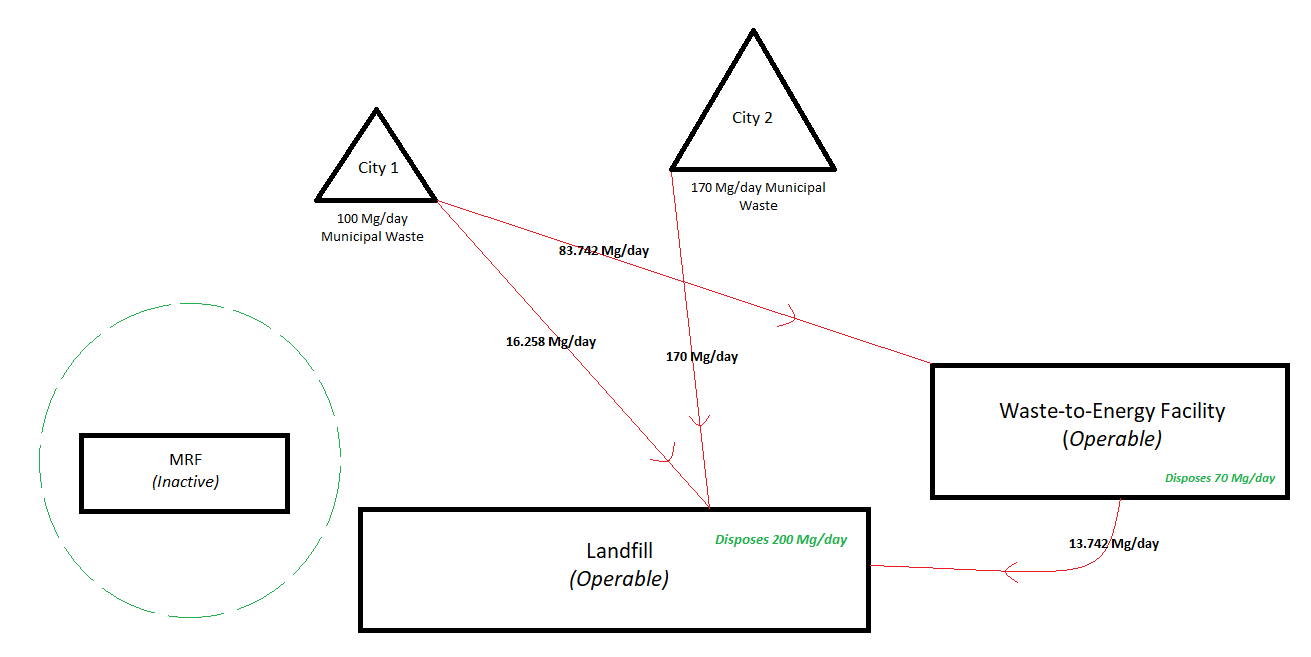
\includegraphics[width=\linewidth]{figures/solution-template_6_1.png}

\section{Problem 2}
\subsection{Problem 2.1}
What the decision variables are will remain unchanged, since the tax would only impact the magnitudes of them. However due to coding limitatons,  notation must change, so the number '2' has been suffixed onto each instance of one. Additionally, the constraints would also stay the same since they only govern physical constraints and capacity limits, but not pricing. The only thing that will signficantly change is the objective, which  needs to be rewritten to incorporate the increased costs of transportation and tipping at the WTE. 

After redoing the math, the governing objective function will remain the same

\[
TC^{2} = Min(C^{2}_{LF}) + C^{2}_{MRF} + C^{2}_{W2E})
\]
But the composition of those will change, specifically the coefficients used in the matrices:

\[
TC^{2} = O^{2}_1 * 2000 + O^{2}_2*1500 + O^{2}_3*2500 + 50*(W^{2}_{1,1}+ W^{2}_{2,1} + R^{2}_{2,1} + R^{2}_{3,1}) + 2.0*(City1[1]*W^{2}_{1,1} + City2[2]*W^{2}_{2,1}) + 7*(W^{2}_{1,2} + W^{2}_{2,2})+ (0.3775*45)*(W^{2}_{1,2} + W^{2}_{2,2})+
2.0*(City1[2]*W^{2}_{1,2} + City2[2]*W^{2}_{2,2} + MRF[1]*R^{2}_{2,1} + MRF[3]*R^{2}_{2,3}) + 75*(W^{2}_{1,3} + W^{2}_{2,3} + R^{2}_{2,3}) + 2.0*(City1[3]*W^{2}_{1,3} + City2[3]*W^{2}_{2,3} + WTE[1]*R^{2}_{3,1})
\]
Changing the objective to: @objective(waste2, Min, sum([2000,1500,2500].\emph{O2) + sum([110 33.9875 105; 100 53.9875 95].}W2) + sum([0 0 0; 114 0 105; 86 0 0].*R2));

\subsection{Problem 2.2}

\begin{lstlisting}
(*@\HLJLk{using}@*) (*@\HLJLn{JuMP}@*)
(*@\HLJLk{using}@*) (*@\HLJLn{Cbc}@*)

(*@\HLJLn{waste2}@*) (*@\HLJLoB{=}@*) (*@\HLJLnf{Model}@*)(*@\HLJLp{(}@*)(*@\HLJLn{Cbc}@*)(*@\HLJLoB{.}@*)(*@\HLJLn{Optimizer}@*)(*@\HLJLp{)}@*)

(*@\HLJLcs{{\#}decision}@*) (*@\HLJLcs{variables}@*)
(*@\HLJLnd{@variable}@*)(*@\HLJLp{(}@*)(*@\HLJLn{waste2}@*)(*@\HLJLp{,}@*) (*@\HLJLn{W2}@*)(*@\HLJLp{[}@*)(*@\HLJLn{i}@*) (*@\HLJLkp{in}@*) (*@\HLJLn{I}@*)(*@\HLJLp{,}@*) (*@\HLJLn{j}@*) (*@\HLJLkp{in}@*) (*@\HLJLn{J}@*)(*@\HLJLp{]}@*) (*@\HLJLoB{\ensuremath{\geq}}@*) (*@\HLJLni{0}@*)(*@\HLJLp{)}@*)
(*@\HLJLnd{@variable}@*)(*@\HLJLp{(}@*)(*@\HLJLn{waste2}@*)(*@\HLJLp{,}@*) (*@\HLJLn{R2}@*)(*@\HLJLp{[}@*)(*@\HLJLn{k}@*) (*@\HLJLkp{in}@*) (*@\HLJLn{J}@*)(*@\HLJLp{,}@*) (*@\HLJLn{j}@*) (*@\HLJLkp{in}@*) (*@\HLJLn{J}@*)(*@\HLJLp{]}@*) (*@\HLJLoB{\ensuremath{\geq}}@*) (*@\HLJLni{0}@*)(*@\HLJLp{)}@*)
(*@\HLJLnd{@variable}@*)(*@\HLJLp{(}@*)(*@\HLJLn{waste2}@*)(*@\HLJLp{,}@*) (*@\HLJLn{O2}@*)(*@\HLJLp{[}@*)(*@\HLJLn{j}@*) (*@\HLJLkp{in}@*) (*@\HLJLn{J}@*)(*@\HLJLp{],}@*) (*@\HLJLn{Bin}@*)(*@\HLJLp{)}@*)

(*@\HLJLcs{{\#}define}@*) (*@\HLJLcs{objective}@*)
(*@\HLJLnd{@objective}@*)(*@\HLJLp{(}@*)(*@\HLJLn{waste2}@*)(*@\HLJLp{,}@*) (*@\HLJLn{Min}@*)(*@\HLJLp{,}@*) (*@\HLJLnf{sum}@*)(*@\HLJLp{([}@*)(*@\HLJLni{2000}@*)(*@\HLJLp{,}@*)(*@\HLJLni{1500}@*)(*@\HLJLp{,}@*)(*@\HLJLni{2500}@*)(*@\HLJLp{]}@*)(*@\HLJLoB{.*}@*)(*@\HLJLn{O2}@*)(*@\HLJLp{)}@*) (*@\HLJLoB{+}@*) (*@\HLJLnf{sum}@*)(*@\HLJLp{([}@*)(*@\HLJLni{110}@*) (*@\HLJLnfB{33.9875}@*) (*@\HLJLni{105}@*)(*@\HLJLp{;}@*) (*@\HLJLni{100}@*) (*@\HLJLnfB{53.9875}@*) (*@\HLJLni{95}@*)(*@\HLJLp{]}@*)(*@\HLJLoB{.*}@*)(*@\HLJLn{W2}@*)(*@\HLJLp{)}@*) (*@\HLJLoB{+}@*) (*@\HLJLnf{sum}@*)(*@\HLJLp{([}@*)(*@\HLJLni{0}@*) (*@\HLJLni{0}@*) (*@\HLJLni{0}@*)(*@\HLJLp{;}@*) (*@\HLJLni{114}@*) (*@\HLJLni{0}@*) (*@\HLJLni{105}@*)(*@\HLJLp{;}@*) (*@\HLJLni{86}@*) (*@\HLJLni{0}@*) (*@\HLJLni{0}@*)(*@\HLJLp{]}@*)(*@\HLJLoB{.*}@*)(*@\HLJLn{R2}@*)(*@\HLJLp{));}@*)

(*@\HLJLcs{{\#}Constraints}@*)
(*@\HLJLcs{{\#}Capacity}@*) (*@\HLJLcs{and}@*) (*@\HLJLcs{input}@*) (*@\HLJLcs{constraints}@*)
(*@\HLJLnd{@constraint}@*)(*@\HLJLp{(}@*)(*@\HLJLn{waste2}@*)(*@\HLJLp{,}@*) (*@\HLJLn{LF}@*)(*@\HLJLp{,}@*) (*@\HLJLn{W2}@*)(*@\HLJLp{[}@*)(*@\HLJLni{1}@*)(*@\HLJLp{,}@*)(*@\HLJLni{1}@*)(*@\HLJLp{]}@*) (*@\HLJLoB{+}@*) (*@\HLJLn{W2}@*)(*@\HLJLp{[}@*)(*@\HLJLni{2}@*)(*@\HLJLp{,}@*)(*@\HLJLni{1}@*)(*@\HLJLp{]}@*) (*@\HLJLoB{+}@*) (*@\HLJLn{R2}@*)(*@\HLJLp{[}@*)(*@\HLJLni{2}@*)(*@\HLJLp{,}@*)(*@\HLJLni{1}@*)(*@\HLJLp{]}@*) (*@\HLJLoB{+}@*) (*@\HLJLn{R2}@*)(*@\HLJLp{[}@*)(*@\HLJLni{3}@*)(*@\HLJLp{,}@*)(*@\HLJLni{1}@*)(*@\HLJLp{]}@*) (*@\HLJLoB{\ensuremath{\leq}}@*) (*@\HLJLni{200}@*)(*@\HLJLp{);}@*)
(*@\HLJLnd{@constraint}@*)(*@\HLJLp{(}@*)(*@\HLJLn{waste2}@*)(*@\HLJLp{,}@*) (*@\HLJLn{MRF}@*)(*@\HLJLp{,}@*) (*@\HLJLn{W2}@*)(*@\HLJLp{[}@*)(*@\HLJLni{1}@*)(*@\HLJLp{,}@*)(*@\HLJLni{2}@*)(*@\HLJLp{]}@*) (*@\HLJLoB{+}@*) (*@\HLJLn{W2}@*)(*@\HLJLp{[}@*)(*@\HLJLni{2}@*)(*@\HLJLp{,}@*)(*@\HLJLni{2}@*)(*@\HLJLp{]}@*) (*@\HLJLoB{\ensuremath{\leq}}@*) (*@\HLJLni{350}@*)(*@\HLJLp{);}@*)
(*@\HLJLnd{@constraint}@*)(*@\HLJLp{(}@*)(*@\HLJLn{waste2}@*)(*@\HLJLp{,}@*) (*@\HLJLn{W2E}@*)(*@\HLJLp{,}@*) (*@\HLJLn{W2}@*)(*@\HLJLp{[}@*)(*@\HLJLni{1}@*)(*@\HLJLp{,}@*)(*@\HLJLni{3}@*)(*@\HLJLp{]}@*) (*@\HLJLoB{+}@*) (*@\HLJLn{W2}@*)(*@\HLJLp{[}@*)(*@\HLJLni{2}@*)(*@\HLJLp{,}@*)(*@\HLJLni{3}@*)(*@\HLJLp{]}@*) (*@\HLJLoB{+}@*) (*@\HLJLn{R2}@*)(*@\HLJLp{[}@*)(*@\HLJLni{2}@*)(*@\HLJLp{,}@*)(*@\HLJLni{3}@*)(*@\HLJLp{]}@*) (*@\HLJLoB{\ensuremath{\leq}}@*) (*@\HLJLni{150}@*)(*@\HLJLp{);}@*)
(*@\HLJLnd{@constraint}@*)(*@\HLJLp{(}@*)(*@\HLJLn{waste2}@*)(*@\HLJLp{,}@*) (*@\HLJLn{MSW}@*)(*@\HLJLp{[}@*)(*@\HLJLn{i}@*) (*@\HLJLkp{in}@*) (*@\HLJLn{I}@*)(*@\HLJLp{],}@*) (*@\HLJLnf{sum}@*)(*@\HLJLp{(}@*)(*@\HLJLn{W2}@*)(*@\HLJLp{[}@*)(*@\HLJLn{i}@*)(*@\HLJLp{,}@*)(*@\HLJLoB{:}@*)(*@\HLJLp{])}@*) (*@\HLJLoB{==}@*) (*@\HLJLn{DSW}@*)(*@\HLJLp{[}@*)(*@\HLJLn{i}@*)(*@\HLJLp{]);}@*)

(*@\HLJLcs{{\#}If}@*) (*@\HLJLcs{no}@*) (*@\HLJLcs{waste}@*) (*@\HLJLcs{servicing,}@*) (*@\HLJLcs{turn}@*) (*@\HLJLcs{off}@*) (*@\HLJLcs{fixed}@*) (*@\HLJLcs{cost}@*)
(*@\HLJLnd{@constraint}@*)(*@\HLJLp{(}@*)(*@\HLJLn{waste2}@*)(*@\HLJLp{,}@*) (*@\HLJLn{open1}@*)(*@\HLJLp{,}@*) (*@\HLJLn{O2}@*)(*@\HLJLp{[}@*)(*@\HLJLni{1}@*)(*@\HLJLp{]}@*) (*@\HLJLoB{==}@*) (*@\HLJLni{1}@*)(*@\HLJLp{)}@*)
(*@\HLJLnd{@constraint}@*)(*@\HLJLp{(}@*)(*@\HLJLn{waste2}@*)(*@\HLJLp{,}@*) (*@\HLJLn{open2}@*)(*@\HLJLp{,}@*) (*@\HLJLoB{!}@*)(*@\HLJLn{O2}@*)(*@\HLJLp{[}@*)(*@\HLJLni{2}@*)(*@\HLJLp{]}@*) (*@\HLJLoB{=>}@*) (*@\HLJLp{{\{}}@*)(*@\HLJLn{W2}@*)(*@\HLJLp{[}@*)(*@\HLJLni{1}@*)(*@\HLJLp{,}@*)(*@\HLJLni{2}@*)(*@\HLJLp{]}@*) (*@\HLJLoB{+}@*) (*@\HLJLn{W2}@*)(*@\HLJLp{[}@*)(*@\HLJLni{2}@*)(*@\HLJLp{,}@*)(*@\HLJLni{2}@*)(*@\HLJLp{]}@*) (*@\HLJLoB{==}@*) (*@\HLJLni{0}@*)(*@\HLJLp{{\}})}@*)
(*@\HLJLnd{@constraint}@*)(*@\HLJLp{(}@*)(*@\HLJLn{waste2}@*)(*@\HLJLp{,}@*) (*@\HLJLn{open3}@*)(*@\HLJLp{,}@*) (*@\HLJLoB{!}@*)(*@\HLJLn{O2}@*)(*@\HLJLp{[}@*)(*@\HLJLni{3}@*)(*@\HLJLp{]}@*) (*@\HLJLoB{=>}@*) (*@\HLJLp{{\{}}@*)(*@\HLJLn{W2}@*)(*@\HLJLp{[}@*)(*@\HLJLni{1}@*)(*@\HLJLp{,}@*)(*@\HLJLni{3}@*)(*@\HLJLp{]}@*) (*@\HLJLoB{+}@*) (*@\HLJLn{W2}@*)(*@\HLJLp{[}@*)(*@\HLJLni{2}@*)(*@\HLJLp{,}@*)(*@\HLJLni{3}@*)(*@\HLJLp{]}@*) (*@\HLJLoB{+}@*) (*@\HLJLn{R2}@*)(*@\HLJLp{[}@*)(*@\HLJLni{2}@*)(*@\HLJLp{,}@*)(*@\HLJLni{3}@*)(*@\HLJLp{]}@*) (*@\HLJLoB{==}@*) (*@\HLJLni{0}@*)(*@\HLJLp{{\}})}@*)

(*@\HLJLcs{{\#}Mass}@*) (*@\HLJLcs{balance}@*) (*@\HLJLcs{constraints}@*)

(*@\HLJLnd{@constraint}@*)(*@\HLJLp{(}@*)(*@\HLJLn{waste2}@*)(*@\HLJLp{,}@*)(*@\HLJLn{RR1}@*)(*@\HLJLp{,}@*) (*@\HLJLnf{sum}@*)(*@\HLJLp{(}@*)(*@\HLJLn{R2}@*)(*@\HLJLp{[}@*)(*@\HLJLni{1}@*)(*@\HLJLp{,}@*)(*@\HLJLoB{:}@*)(*@\HLJLp{])}@*)(*@\HLJLoB{==}@*) (*@\HLJLni{0}@*)(*@\HLJLp{)}@*)
(*@\HLJLnd{@constraint}@*)(*@\HLJLp{(}@*)(*@\HLJLn{waste2}@*)(*@\HLJLp{,}@*) (*@\HLJLn{RR2}@*)(*@\HLJLp{,}@*) (*@\HLJLn{R2}@*)(*@\HLJLp{[}@*)(*@\HLJLni{2}@*)(*@\HLJLp{,}@*)(*@\HLJLni{3}@*)(*@\HLJLp{]}@*) (*@\HLJLoB{+}@*) (*@\HLJLn{R2}@*)(*@\HLJLp{[}@*)(*@\HLJLni{2}@*)(*@\HLJLp{,}@*)(*@\HLJLni{1}@*)(*@\HLJLp{]}@*) (*@\HLJLoB{==}@*) (*@\HLJLp{(}@*)(*@\HLJLni{1}@*)(*@\HLJLoB{-}@*)(*@\HLJLn{XX}@*)(*@\HLJLp{)}@*)(*@\HLJLoB{*}@*)(*@\HLJLp{(}@*)(*@\HLJLn{W2}@*)(*@\HLJLp{[}@*)(*@\HLJLni{1}@*)(*@\HLJLp{,}@*)(*@\HLJLni{2}@*)(*@\HLJLp{]}@*)(*@\HLJLoB{+}@*)(*@\HLJLn{W2}@*)(*@\HLJLp{[}@*)(*@\HLJLni{2}@*)(*@\HLJLp{,}@*)(*@\HLJLni{2}@*)(*@\HLJLp{]))}@*)
(*@\HLJLnd{@constraint}@*)(*@\HLJLp{(}@*)(*@\HLJLn{waste2}@*)(*@\HLJLp{,}@*) (*@\HLJLn{RR3}@*)(*@\HLJLp{,}@*) (*@\HLJLn{R2}@*)(*@\HLJLp{[}@*)(*@\HLJLni{3}@*)(*@\HLJLp{,}@*)(*@\HLJLni{1}@*)(*@\HLJLp{]}@*) (*@\HLJLoB{==}@*) (*@\HLJLn{YY}@*)(*@\HLJLoB{*}@*)(*@\HLJLp{(}@*)(*@\HLJLn{W2}@*)(*@\HLJLp{[}@*)(*@\HLJLni{1}@*)(*@\HLJLp{,}@*)(*@\HLJLni{3}@*)(*@\HLJLp{]}@*)(*@\HLJLoB{+}@*)(*@\HLJLn{W2}@*)(*@\HLJLp{[}@*)(*@\HLJLni{2}@*)(*@\HLJLp{,}@*)(*@\HLJLni{3}@*)(*@\HLJLp{])}@*) (*@\HLJLoB{+}@*) (*@\HLJLn{NewAshContent}@*)(*@\HLJLoB{*}@*)(*@\HLJLp{(}@*)(*@\HLJLn{R2}@*)(*@\HLJLp{[}@*)(*@\HLJLni{2}@*)(*@\HLJLp{,}@*)(*@\HLJLni{3}@*)(*@\HLJLp{]))}@*)
(*@\HLJLnd{@constraint}@*)(*@\HLJLp{(}@*)(*@\HLJLn{waste2}@*)(*@\HLJLp{,}@*) (*@\HLJLn{SelfServe}@*)(*@\HLJLp{,}@*) (*@\HLJLnf{sum}@*)(*@\HLJLp{(}@*)(*@\HLJLn{R2}@*)(*@\HLJLp{[}@*)(*@\HLJLn{j}@*)(*@\HLJLp{,}@*)(*@\HLJLn{j}@*)(*@\HLJLp{]}@*) (*@\HLJLk{for}@*) (*@\HLJLn{j}@*) (*@\HLJLkp{in}@*) (*@\HLJLn{J}@*)(*@\HLJLp{)}@*) (*@\HLJLoB{==}@*) (*@\HLJLni{0}@*)(*@\HLJLp{)}@*)
(*@\HLJLnd{@constraint}@*)(*@\HLJLp{(}@*)(*@\HLJLn{waste2}@*)(*@\HLJLp{,}@*) (*@\HLJLn{NoReverse}@*)(*@\HLJLp{,}@*) (*@\HLJLn{R2}@*)(*@\HLJLp{[}@*)(*@\HLJLni{3}@*)(*@\HLJLp{,}@*)(*@\HLJLni{2}@*)(*@\HLJLp{]}@*) (*@\HLJLoB{==}@*) (*@\HLJLni{0}@*)(*@\HLJLp{)}@*)


(*@\HLJLcs{{\#}Run}@*) (*@\HLJLcs{code}@*)
(*@\HLJLnf{set{\_}silent}@*)(*@\HLJLp{(}@*)(*@\HLJLn{waste2}@*)(*@\HLJLp{)}@*)
(*@\HLJLnf{optimize!}@*)(*@\HLJLp{(}@*)(*@\HLJLn{waste2}@*)(*@\HLJLp{)}@*)
\end{lstlisting}


\subsection{Problem 2.3}

\begin{lstlisting}
(*@\HLJLn{lowCost2}@*) (*@\HLJLoB{=}@*) (*@\HLJLnf{round}@*)(*@\HLJLp{(}@*)(*@\HLJLnf{objective{\_}value}@*)(*@\HLJLp{(}@*)(*@\HLJLn{waste2}@*)(*@\HLJLp{),}@*) (*@\HLJLn{digits}@*) (*@\HLJLoB{=}@*) (*@\HLJLni{2}@*) (*@\HLJLp{);}@*)
(*@\HLJLnf{println}@*)(*@\HLJLp{(}@*)(*@\HLJLs{"{}The}@*) (*@\HLJLs{New}@*) (*@\HLJLs{Optimal}@*) (*@\HLJLs{Objective}@*) (*@\HLJLs{Value}@*) (*@\HLJLs{is}@*) (*@\HLJLse{{\textbackslash}{\$}}@*)(*@\HLJLs{"{}}@*)(*@\HLJLp{,}@*) (*@\HLJLn{lowCost2}@*)(*@\HLJLp{,}@*)(*@\HLJLs{"{}."{}}@*)(*@\HLJLp{);}@*)
(*@\HLJLnf{println}@*)(*@\HLJLp{(}@*)(*@\HLJLn{value}@*)(*@\HLJLoB{.}@*)(*@\HLJLp{(}@*)(*@\HLJLn{W2}@*)(*@\HLJLp{));}@*)
(*@\HLJLnf{println}@*)(*@\HLJLp{(}@*)(*@\HLJLn{value}@*)(*@\HLJLoB{.}@*)(*@\HLJLp{(}@*)(*@\HLJLn{O2}@*)(*@\HLJLp{));}@*)
(*@\HLJLnf{println}@*)(*@\HLJLp{(}@*)(*@\HLJLn{value}@*)(*@\HLJLoB{.}@*)(*@\HLJLp{(}@*)(*@\HLJLn{R2}@*)(*@\HLJLp{));}@*)
\end{lstlisting}

The New Optimal Objective Value is $33126.95.
2-dimensional DenseAxisArray{Float64,2,...} with index sets:
    Dimension 1, 1:2
    Dimension 2, 1:3
And data, a 2×3 Matrix{Float64}:
  0.0               100.0               0.0
 84.56953642384113   85.43046357615889  0.0
1-dimensional DenseAxisArray{Float64,1,...} with index sets:
    Dimension 1, 1:3
And data, a 3-element Vector{Float64}:
 1.0
 1.0
 0.0
2-dimensional DenseAxisArray{Float64,2,...} with index sets:
    Dimension 1, 1:3
    Dimension 2, 1:3
And data, a 3×3 Matrix{Float64}:
   0.0               0.0  0.0
 115.43046357615891  0.0  0.0
   0.0               0.0  0.0


As a result, now the Waste-to-Energy facility (j = 3) will not be operational, and the MRF and Landfill will be. City 1 will now send all of their waste (100 Mg/day)to the MRF, and City2 will split their 170 Mg/day almost evenly  between the landfill and MRF (84.57 and 85.43 Mg/day, respectively). Of the waste send to the MRF, 115.43 Mg/day will ultimately  still end up in the landfill. 

The primary differences are that now the MRF is operational instead of the Waste-to-Energy facility, and that City2 is no longer sending all of their waste directly to the Landfill, but sending half of it to the MRF first. Ultimately, though, the Landfill still takes on the maxium 200Mg/day in either instance,  reiterating the fact that it still remains the lowest cost method of waste disposal.

Diagram:


\begin{lstlisting}
(*@\HLJLk{using}@*) (*@\HLJLn{Images}@*)(*@\HLJLp{,}@*) (*@\HLJLn{FileIO}@*)
(*@\HLJLn{img{\_}path2}@*)(*@\HLJLoB{=}@*) (*@\HLJLs{"{}C:/Users/Owner/OneDrive}@*) (*@\HLJLs{-}@*) (*@\HLJLs{Cornell}@*) (*@\HLJLs{University/Pictures/BEE4750-HW4-Diagram2.png"{}}@*)
(*@\HLJLn{image2}@*) (*@\HLJLoB{=}@*) (*@\HLJLnf{load}@*)(*@\HLJLp{(}@*)(*@\HLJLn{img{\_}path2}@*)(*@\HLJLp{)}@*)
\end{lstlisting}

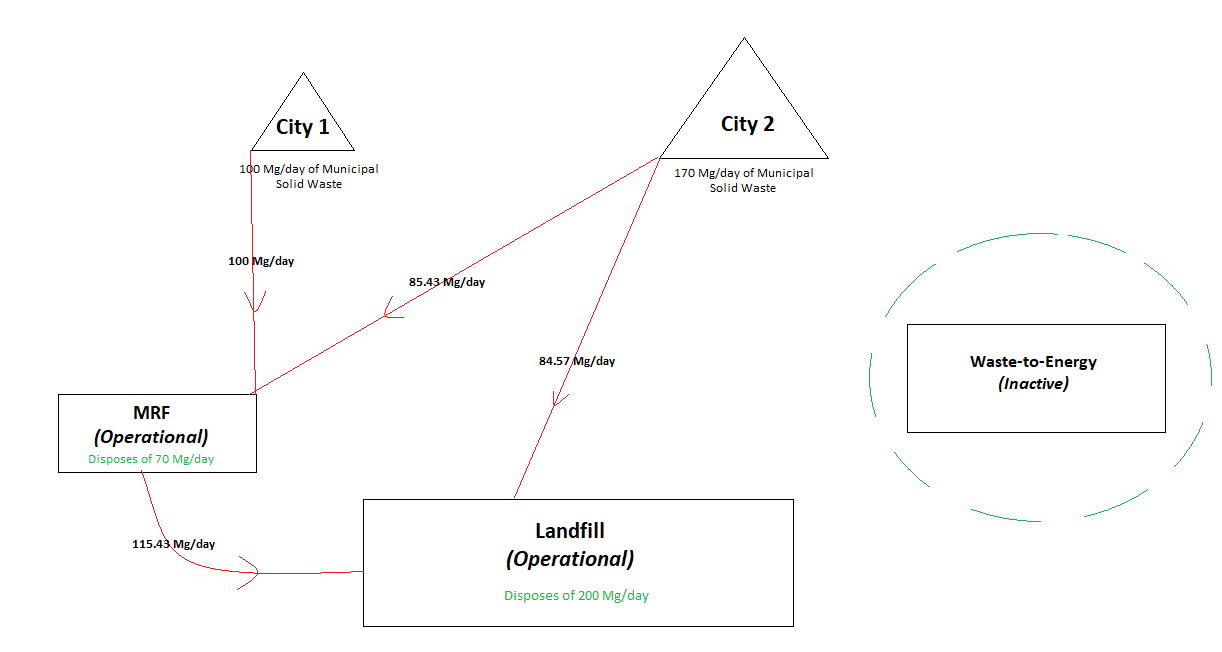
\includegraphics[width=\linewidth]{figures/solution-template_9_1.png}

\section{References}
Help with importing images from file -> https://juliaimages.org/latest/install/ Help with LaTex terminology -> https://www.cmor-faculty.rice.edu/{\textasciitilde}heinken/latex/symbols.pdf



\end{document}